% Created 2023-04-10 Mon 20:51
% Intended LaTeX compiler: xelatex
\documentclass[aspectratio=1610,xcolor={dvipsnames},hyperref={colorlinks,unicode,linkcolor=violet,anchorcolor=BlueViolet,citecolor=YellowOrange,filecolor=black,urlcolor=Aquamarine}]{beamer}
\usepackage{graphicx}
\usepackage{grffile}
\usepackage{longtable}
\usepackage{booktabs}
\usepackage{wrapfig}
\usepackage{rotating}
\usepackage[normalem]{ulem}
\usepackage{amsmath}
\usepackage{textcomp}
\usepackage{amssymb}
\usepackage{capt-of}
\usepackage{nicefrac}
\usepackage[dvipsnames]{xcolor}
\usepackage[colorlinks,unicode,linkcolor=violet,anchorcolor=BlueViolet,citecolor=YellowOrange,filecolor=black,urlcolor=Aquamarine]{hyperref}
\AtBeginSubsection[]{\begin{frame}<beamer>\frametitle{Section}\tableofcontents[currentsection,currentsubsection]\end{frame}}
\synctex=1
\usepackage{etoolbox}
\useoutertheme{infolines}
\setbeamertemplate{frametitle}{%
\usebeamerfont{frametitle}\insertframetitle\strut%
\vskip-0\baselineskip%
\leaders\vrule width .95\paperwidth\vskip1pt%
\vskip0pt%
\nointerlineskip%
}

%% T for footer
\setbeamercolor{footlinecolor}{fg=cyan,bg=green}
\setbeamercolor{author in head/foot}{fg=blue}
\setbeamertemplate{footline}{%
\leavevmode%
\hbox{%
\begin{beamercolorbox}[wd=.26\paperwidth,ht=2.25ex,dp=1ex,left]{author in head/foot}%
\hspace*{2ex}\usebeamerfont{author in head/foot} Dept. CSE, UT Arlington
\end{beamercolorbox}%
\begin{beamercolorbox}[wd=.50\paperwidth,ht=2.25ex,dp=1ex,center]{author in head/foot}%
\usebeamerfont{title in head/foot}Scalable Modeling \& Imaging \& Learning Lab (SMILE)
\end{beamercolorbox}%
\begin{beamercolorbox}[wd=.24\paperwidth,ht=2.25ex,dp=1ex,right]{date in head/foot}%
\usebeamerfont{date in head/foot}
\insertshortdate{}\hspace*{1em}  % date
\insertframenumber/\inserttotalframenumber\hspace*{2ex}
\end{beamercolorbox}}%
\vskip0pt%
}
\setbeamerfont{footnote}{size=\tiny}
\usepackage{minted}
\setbeamerfont{caption}{size=\scriptsize}
\usetheme{default}
\usefonttheme{serif}
\useinnertheme{circles}
\author{Nasy}
\date{Mar 24, 2023}
\title{In-Context Learning -- Human-Computer Interface}
\hypersetup{
 pdfauthor={Nasy},
 pdftitle={In-Context Learning -- Human-Computer Interface},
 pdfkeywords={},
 pdfsubject={},
 pdfcreator={Emacs 29.0.50 (Org mode 9.5.5)}, 
 pdflang={English}}
\usepackage{biblatex}
\addbibresource{/Users/Nasy/.emacs.d/萚兮/時/refs/ref.bib}
\begin{document}

\maketitle
\begin{frame}{Outline}
\setcounter{tocdepth}{1}
\tableofcontents
\end{frame}

\setcounter{tocdepth}{2}

\section{Introduction}
\label{sec:orgb735d61}

\begin{frame}[label={sec:org5c3e51a},fragile]{Example -- Transfrom a table to a review sentiment template}
 Table:

\begin{center}
\begin{tabular}{lr}
\toprule
Text & Label\\[0pt]
\midrule
Delicious food & 1\\[0pt]
The food is awful & 0\\[0pt]
Terrible dishes & 0\\[0pt]
\bottomrule
\end{tabular}
\end{center}

Template: Review: [text] Sentiment: [label]

\begin{verbatim}
[ME]:
Review: Delicious food      Sentiment: Positive
Review: The food is awful   Sentiment: Negative
Review: Terrible dishes     Sentiment: Negative
Review: Good meal           Sentiment:
[AI]: Positive
\end{verbatim}
\end{frame}

\begin{frame}[label={sec:org99f6144}]{Example -- Emoji}
\begin{figure}[htbp]
\centering
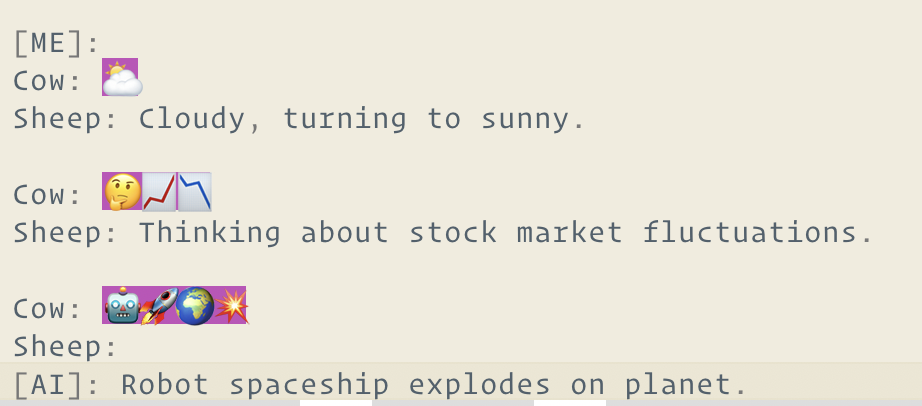
\includegraphics[width=.9\linewidth]{./pex1.png}
\caption{\label{fig:org68b9ee0}Emoji English translation.}
\end{figure}
\end{frame}

\begin{frame}[label={sec:org43ea0fe}]{Example -- Graph}
See org file
\end{frame}

\section{In-Context Learning}
\label{sec:orga016819}

\subsection{Definition}
\label{sec:orgd9c8903}

\begin{frame}[label={sec:org56d5c7d}]{Definition}
\begin{description}
\item[{Input}] A demonstration set \(C = \{<x_{i}, y_{i}> | i \in [1, n]\}\), and the next \(x_{n+1}\)
\item[{Output}] \(y_{n+1}\)
\end{description}

\[P( y_{j} | x ) = f_{M}(y_{i}, x_{i}, C), i \in [1, n] \]
\[ y_{n + 1} = \operatorname*{arg\,max}_{y_{j}} P(y_{j}|x) \]
\end{frame}

\begin{frame}[label={sec:org0e6c92b},fragile]{Difference between ICL and others}
 \begin{center}
\begin{tabular}{llll}
\toprule
 & Model & Task description & Examples\\[0pt]
\midrule
Fine-tune & Update & Yes & Yes\\[0pt]
Few-shot & Original & Yes & Yes\\[0pt]
Zero-shot (Instruct) & Original & Yes & No\\[0pt]
In-Context Learning & Original & No & Yes\\[0pt]
\bottomrule
\end{tabular}
\end{center}

{\tiny

\begin{verbatim}
[ME]:
### Transform sentence to triplets.  // Task description (Instruct)

### E.g.
Alice is Bob’s roommate. Make her node green.
[
["Alice", "is roommate", "Bob"],
["Alice", "#00FF00"]
]

### Input
Over-fitting and over-smoothing are two main obstacles of developing deep Graph Convolutional Networks (GCNs) for node classification.

[AI]: [
["over-fitting", "are obstacles of", "developing deep Graph Convolutional Networks for node classification"],
["over-smoothing", "are obstacles of", "developing deep Graph Convolutional Networks for node classification"]
]
\end{verbatim}

}
\end{frame}

\subsection{Taxonomy}
\label{sec:orgf70e7a9}

\begin{frame}[label={sec:org4068af3}]{Taxonomy of in-context learning.}
ICL Paper list: \url{https://github.com/dqxiu/ICL\_PaperList}

\begin{figure}[htbp]
\centering
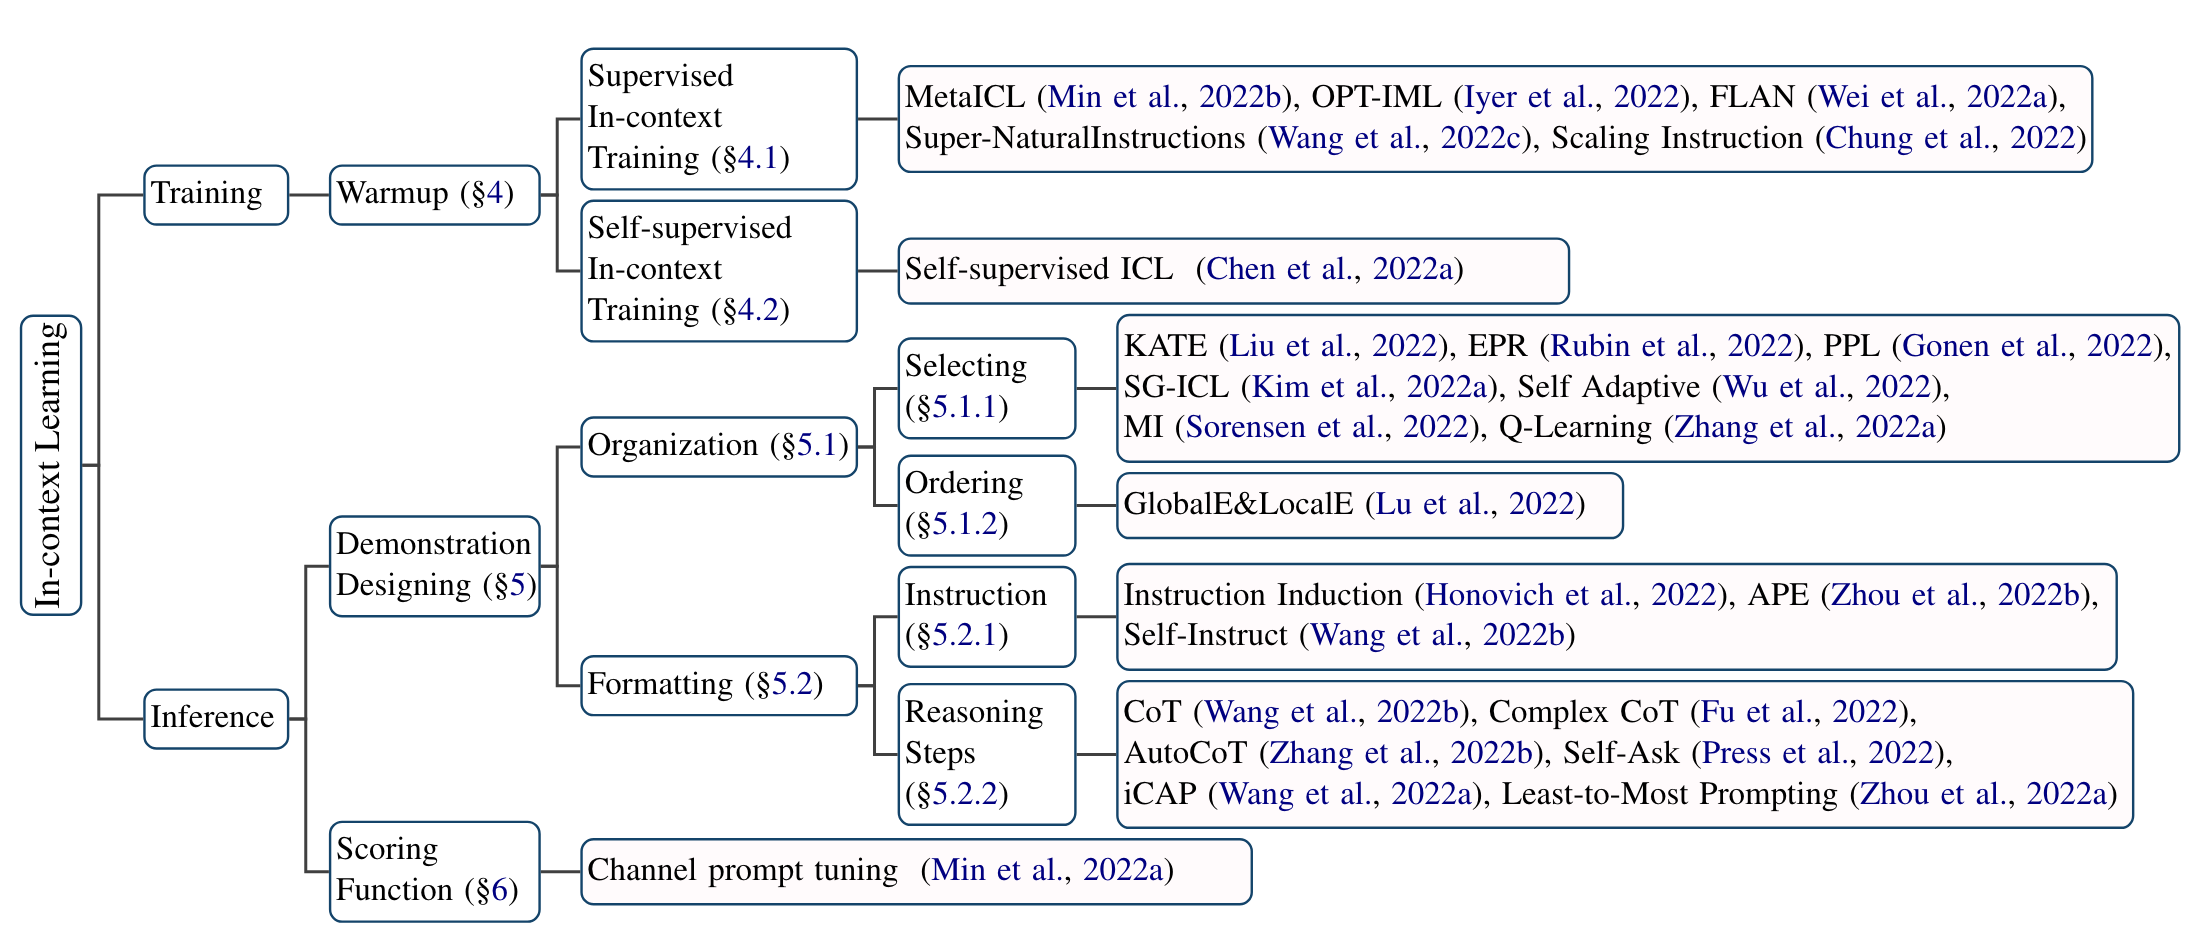
\includegraphics[width=.9\linewidth]{./p1.png}
\caption{\label{fig:org92c327c}Taxonomy of in-context learning \footfullcite{dongSurveyIncontextLearning2023}.}
\end{figure}
\end{frame}

\begin{frame}[label={sec:org20c7918}]{Large Language Models Are Human-Level Prompt Engineers}
\tiny If we assume that In-Context Learning is the use of examples to concretely express task commands, and Instruct is a more abstract task description that is better suited to human habits, then a very natural question is: what is the connection between them?

\begin{figure}[htbp]
\centering
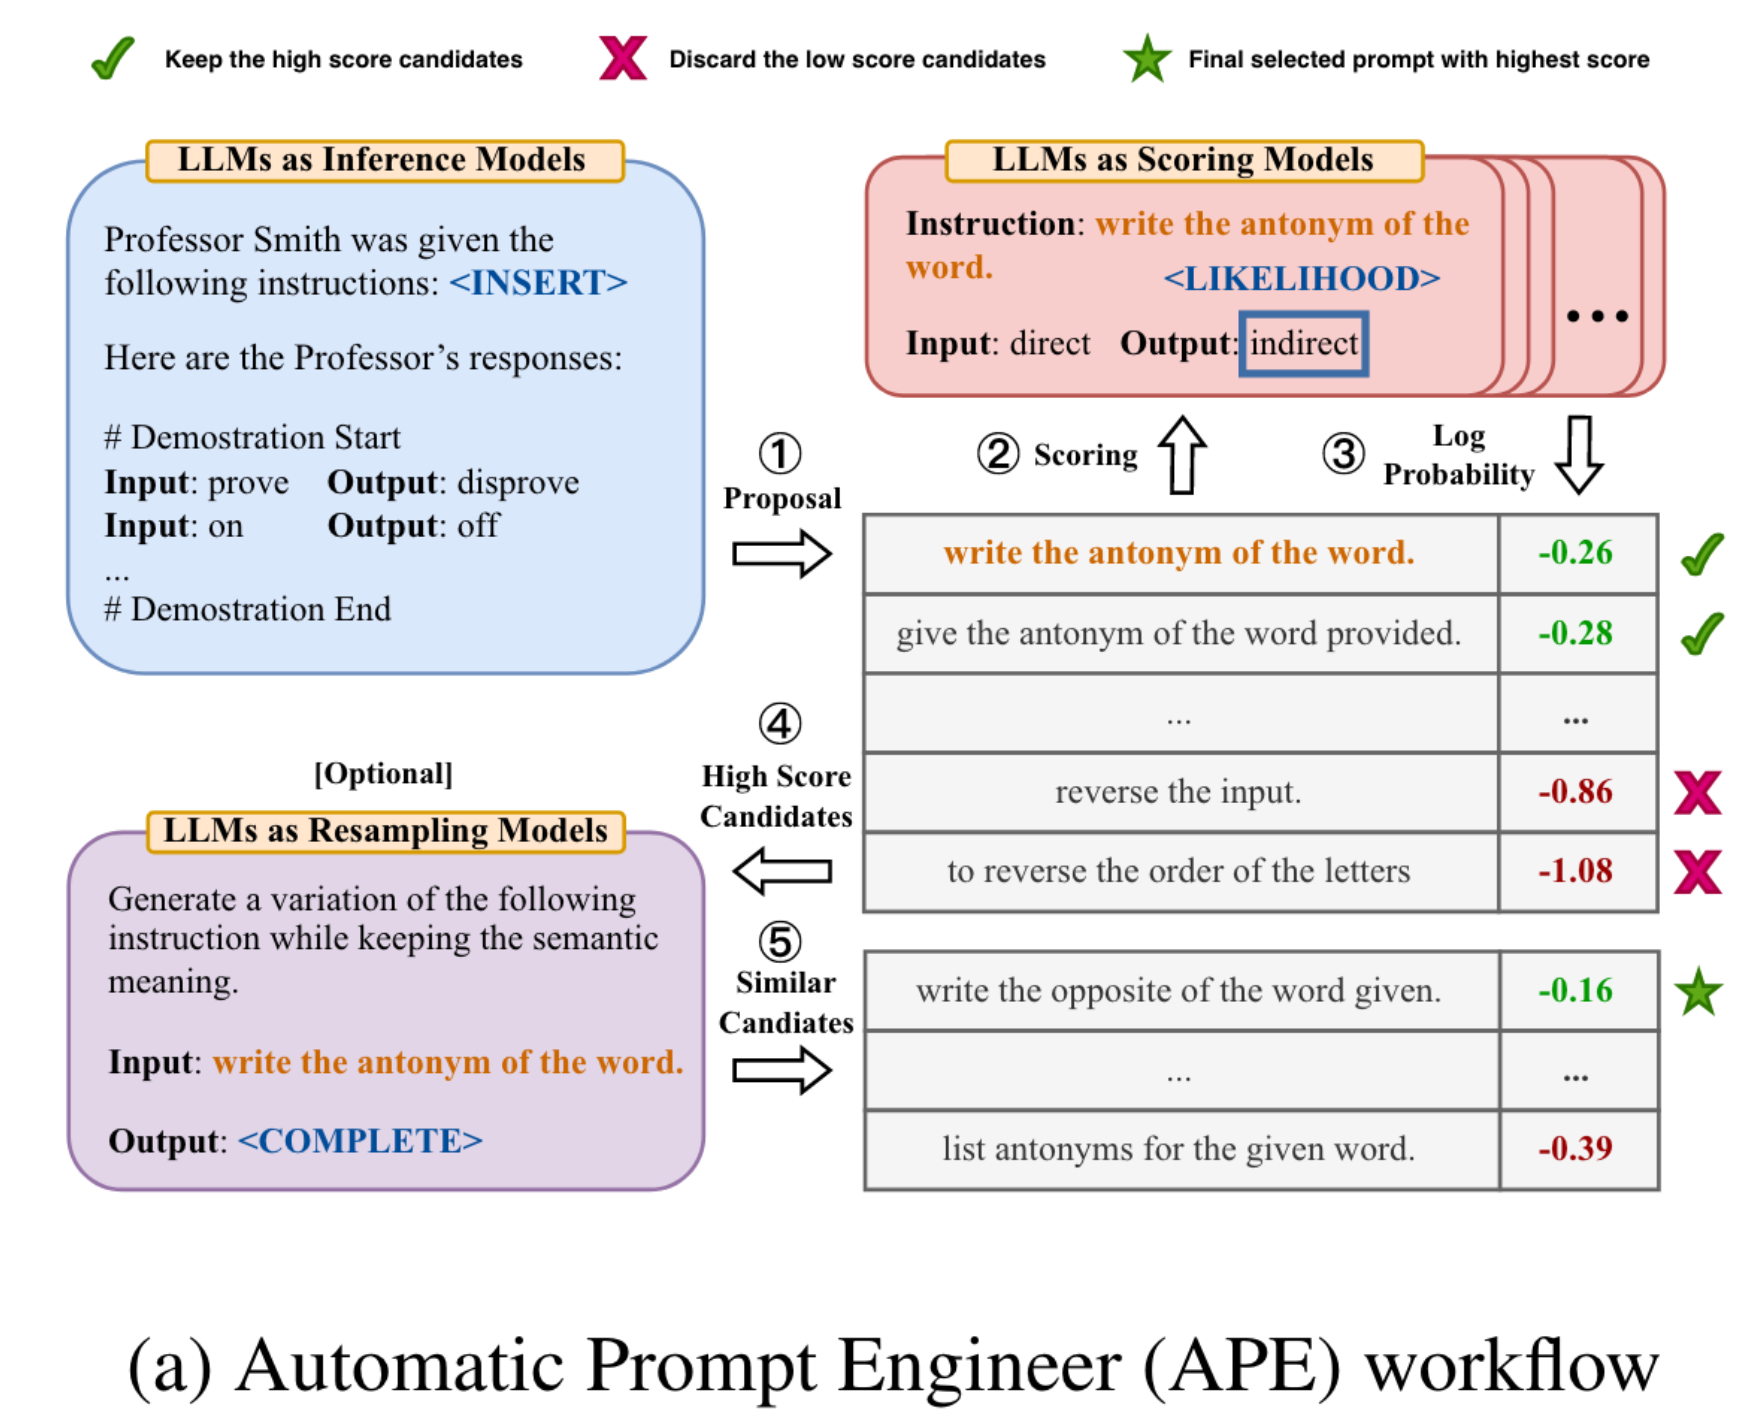
\includegraphics[height=6cm]{./p9.png}
\caption{\label{fig:org00e32be}\tiny Automatic Prompt Engineer (APE) workflow \footfullcite{zhouLargeLanguageModels2023}. Demo: \url{https://sites.google.com/view/automatic-prompt-engineer}}
\end{figure}
\end{frame}

\subsection{Training}
\label{sec:orgb2ada29}

\begin{frame}[label={sec:orga32f7bd}]{Training}
During training, split the raw text into ICL examples.  As the data size increases, the effect gradually flattens out, but increasing task diversity can further enhance performance.

\begin{figure}[htbp]
\centering
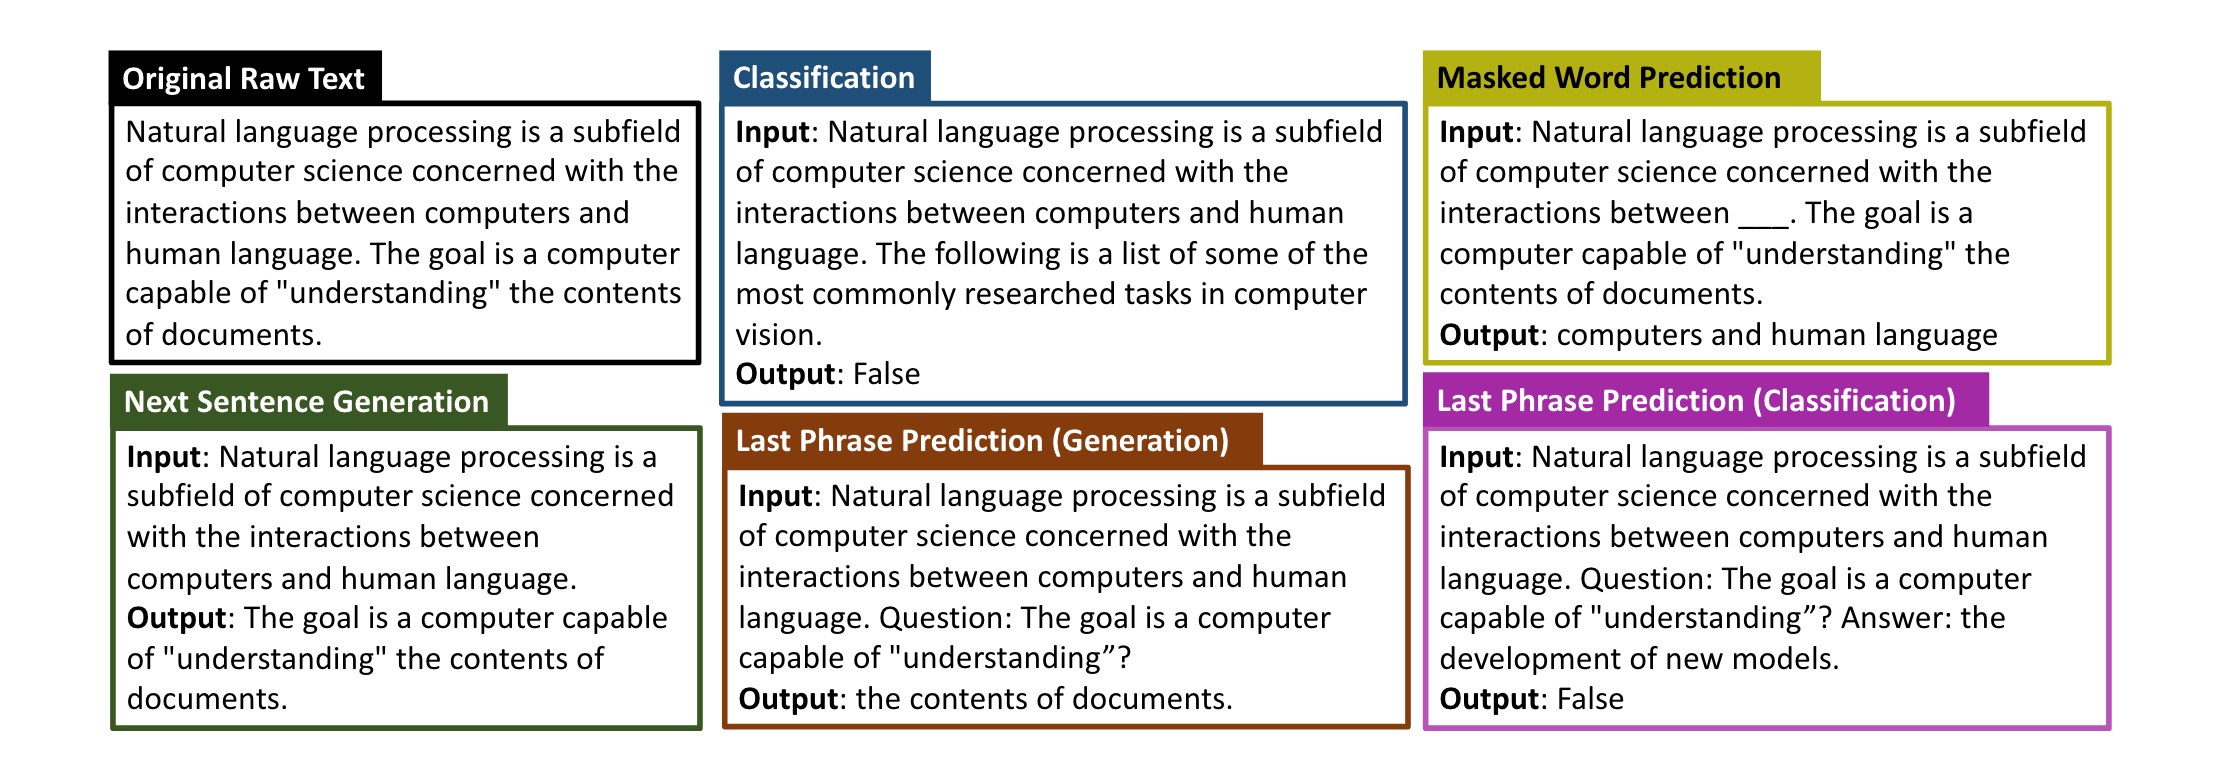
\includegraphics[width=.9\linewidth]{./p2.png}
\caption{\label{fig:orgb827582}Each example is an input-output pair constructed from the raw text. \footfullcite{chenImprovingInContextFewShot2022}}
\end{figure}
\end{frame}

\subsection{Inference}
\label{sec:org26a4982}

\begin{frame}[label={sec:org1417a51}]{Inference -- Demonstration Designing}
\begin{itemize}
\item Demostration Organization
\begin{itemize}
\item Selection
\item Order
\end{itemize}
\item Demostration Formatting
\begin{itemize}
\item Instruction
\item Reasoning Steps
\end{itemize}
\end{itemize}
\end{frame}

\begin{frame}[label={sec:orga214039}]{Selection and Order}
\begin{description}
\item[{Target}] Which examples are good examples for ICL?
\end{description}

\begin{columns}
\begin{column}{0.4\columnwidth}
\begin{itemize}
\item Unsupervised Method
\begin{itemize}
\item L2 distance
\item Cosine similarity
\item \ldots{}
\item LLM
\end{itemize}
\item Supervised Method
\begin{itemize}
\item Human Feedback Reinforcement Learning
\item \ldots{}
\end{itemize}
\end{itemize}
\end{column}

\begin{column}{0.4\columnwidth}
\begin{itemize}
\item Put the most similar examples last.
\item Order by entropy metrics \footfullcite{luFantasticallyOrderedPrompts2022}
\end{itemize}
\end{column}
\end{columns}
\end{frame}

\begin{frame}[label={sec:org9c243b3}]{Formatting}
\begin{itemize}
\item Instruction
\begin{itemize}
\item Finetuned Language Models are Zero-Shot Learners (FLAN) \footfullcite{weiFinetunedLanguageModels2022}
\end{itemize}
\item Reasoning Steps
\begin{itemize}
\item CoT (Chain of Thought) \footfullcite{weiChainofThoughtPromptingElicits2022}
\item Self-consistency \footfullcite{wangSelfConsistencyImprovesChain2023}
\item Least-to-most prompting \footfullcite{zhouLeasttoMostPromptingEnables2023}
\item Lets think step by step (Zero-Shot-CoT) \footfullcite{kojimaLargeLanguageModels2023}
\end{itemize}
\end{itemize}
\end{frame}

\begin{frame}[label={sec:orgc653b00}]{FLAN \footfullcite{weiFinetunedLanguageModels2022}}
\begin{figure}[htbp]
\centering
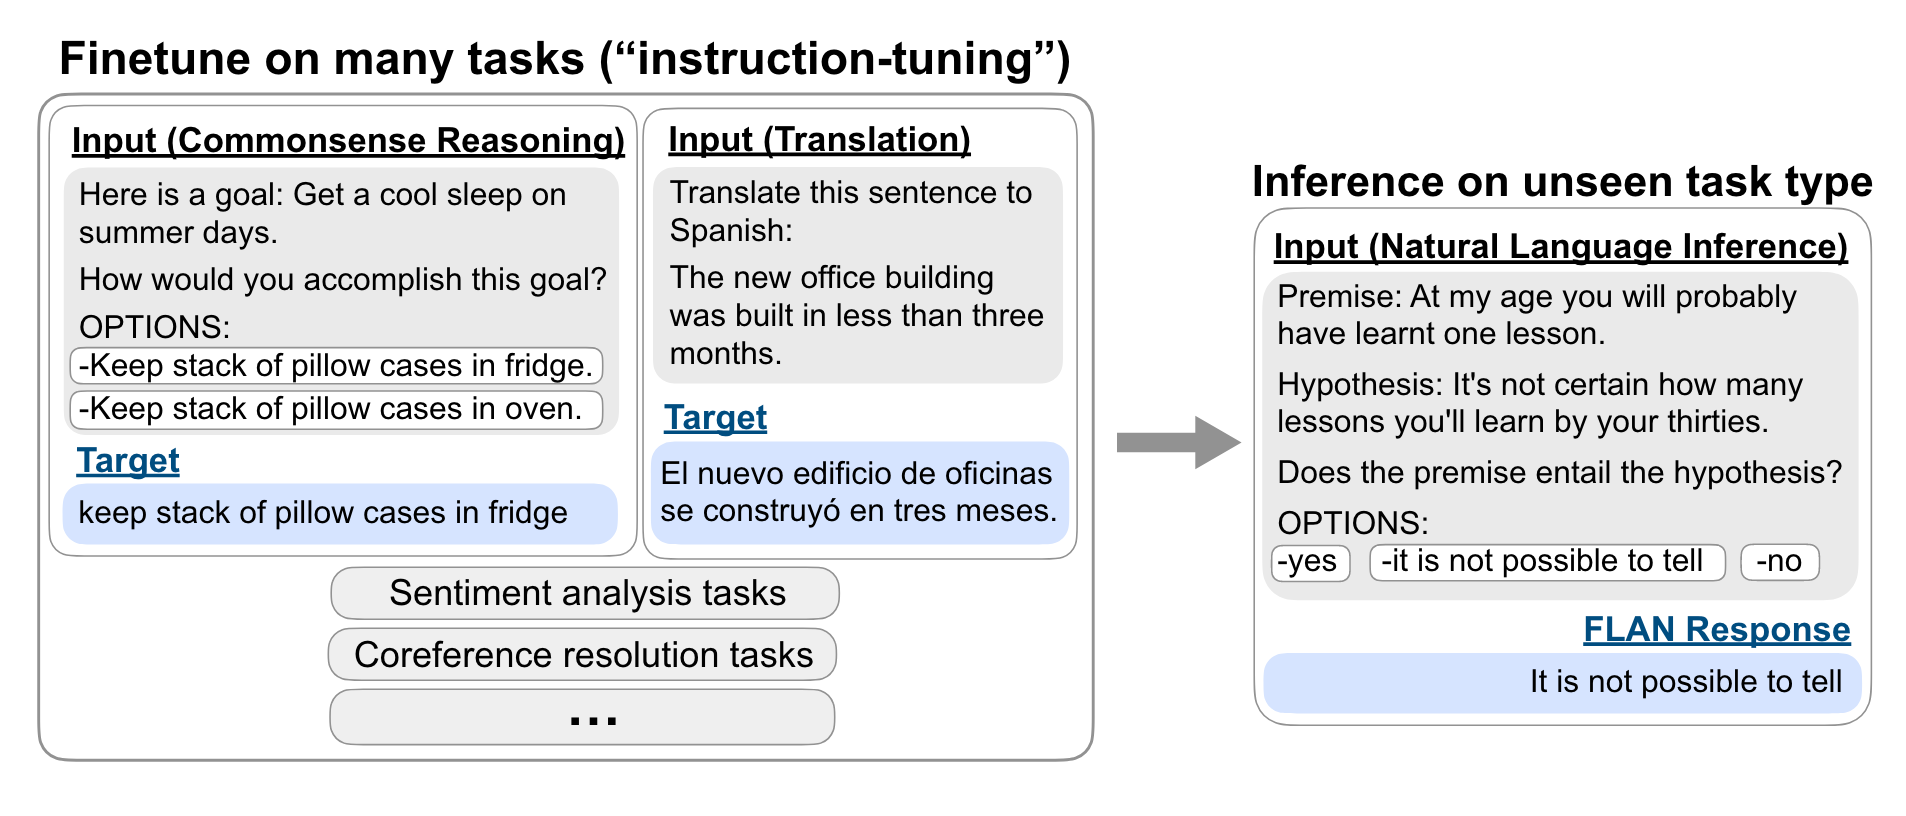
\includegraphics[height=6cm]{./p6.png}
\caption{\label{fig:org387cbf6}Instruction tuning finetunes a pretrained language model on a mixture of tasks phrased as instructions.}
\end{figure}
\end{frame}

\begin{frame}[label={sec:org6aff90f}]{CoT \footfullcite{weiChainofThoughtPromptingElicits2022}.}
\begin{figure}[htbp]
\centering
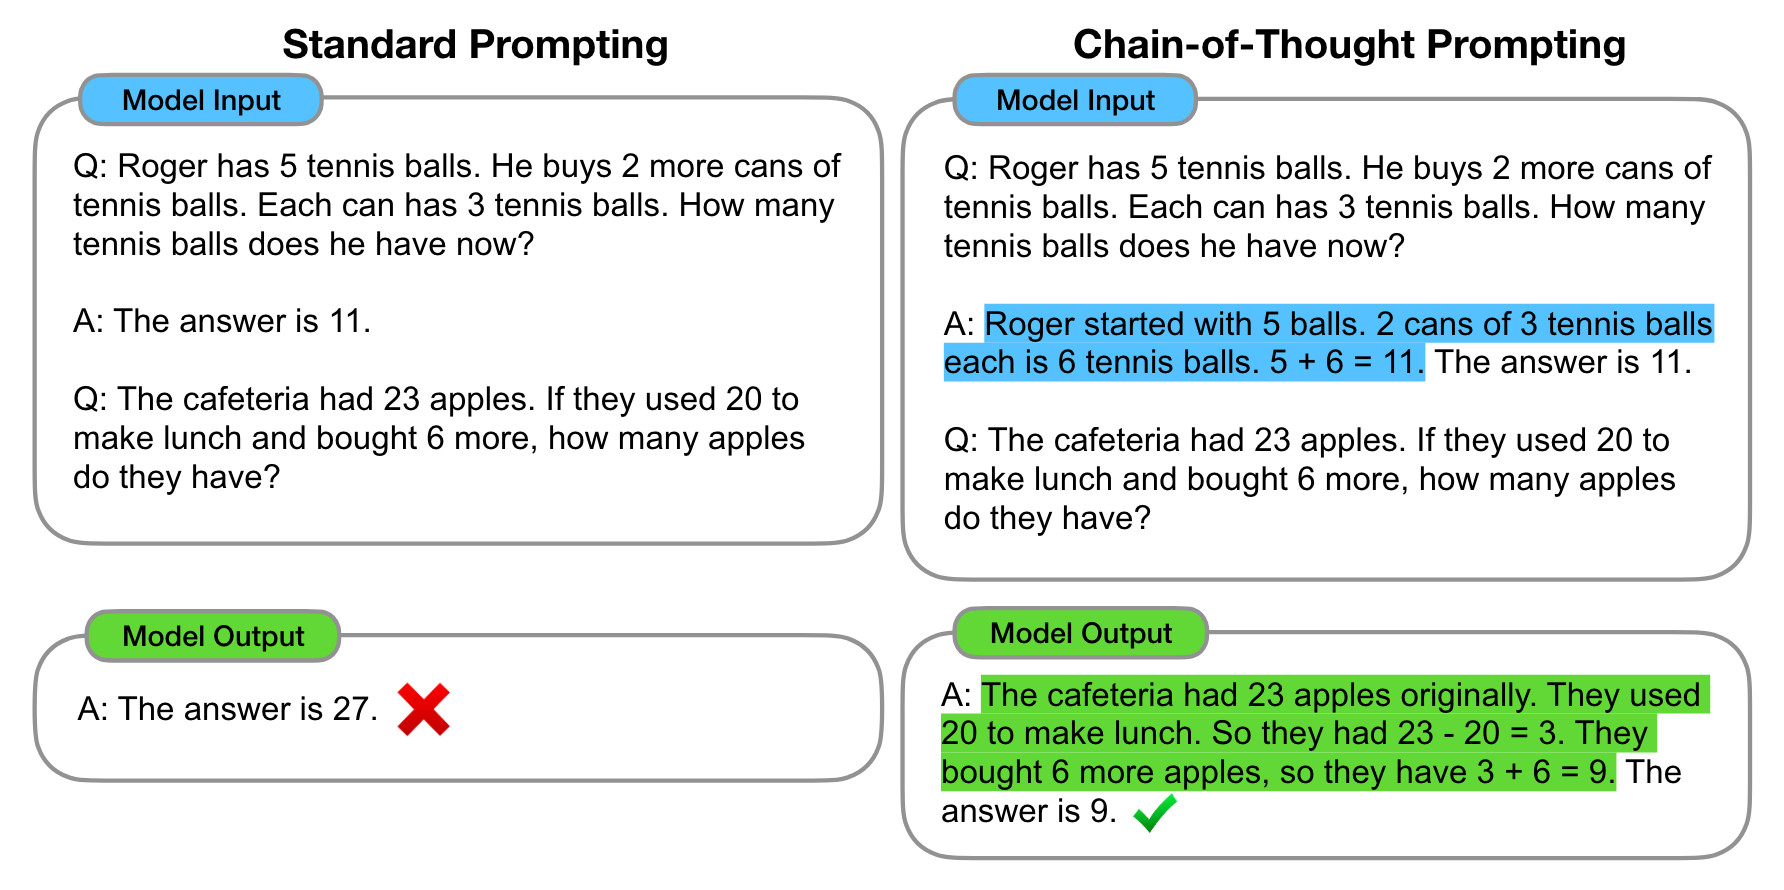
\includegraphics[height=6.2cm]{./p3.png}
\caption{\label{fig:org7b32b6a}\tiny Chain-of-thought prompting enables large language models to tackle complex arithmetic, commonsense, and symbolic reasoning tasks.  Chain-of-thought reasoning processes are highlighted.}
\end{figure}
\end{frame}

\begin{frame}[label={sec:org9f743c1}]{Self Consistency \footfullcite{wangSelfConsistencyImprovesChain2023}}
\begin{figure}[htbp]
\centering
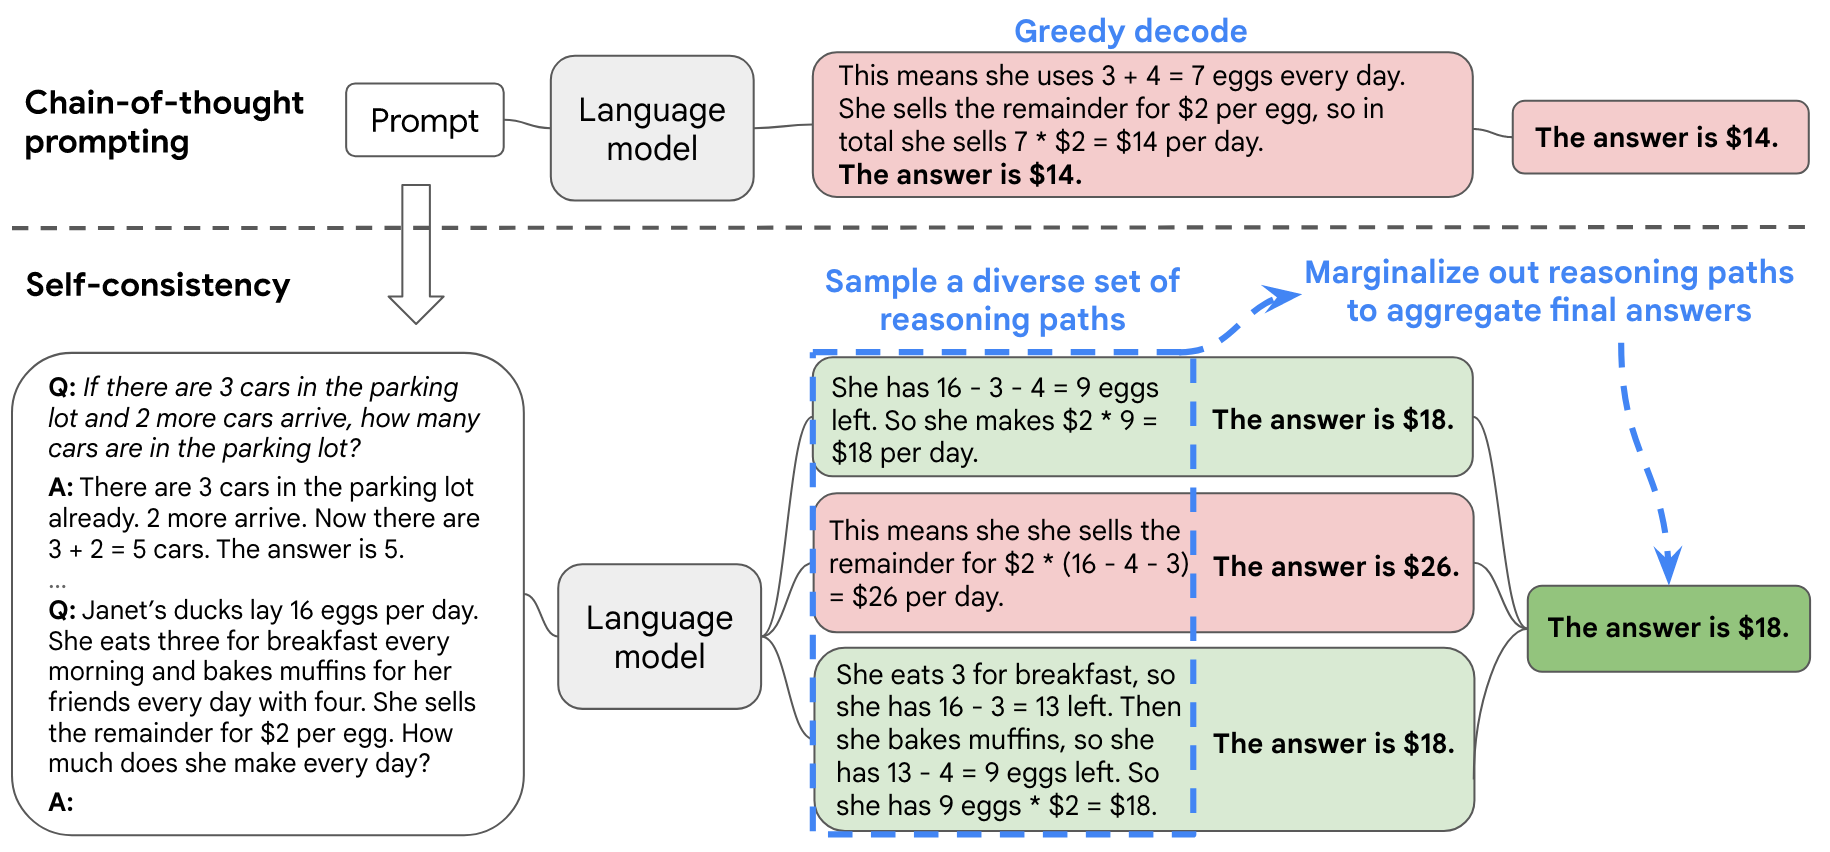
\includegraphics[height=6.2cm]{./p7.png}
\caption{\label{fig:org4674144}\tiny The self-consistency method contains three steps: (1) prompt a language model using chain-of-thought (CoT) prompting; (2) replace the “greedy decode” in CoT prompting by sampling from the language model’s decoder to generate a diverse set of reasoning paths; and (3) marginalize out the reasoning paths and aggregate by choosing the most consistent answer in the final answer set.}
\end{figure}
\end{frame}

\begin{frame}[label={sec:orgf2d17ed}]{Least-to-most prompting \footfullcite{zhouLeasttoMostPromptingEnables2023}}
\begin{figure}[htbp]
\centering
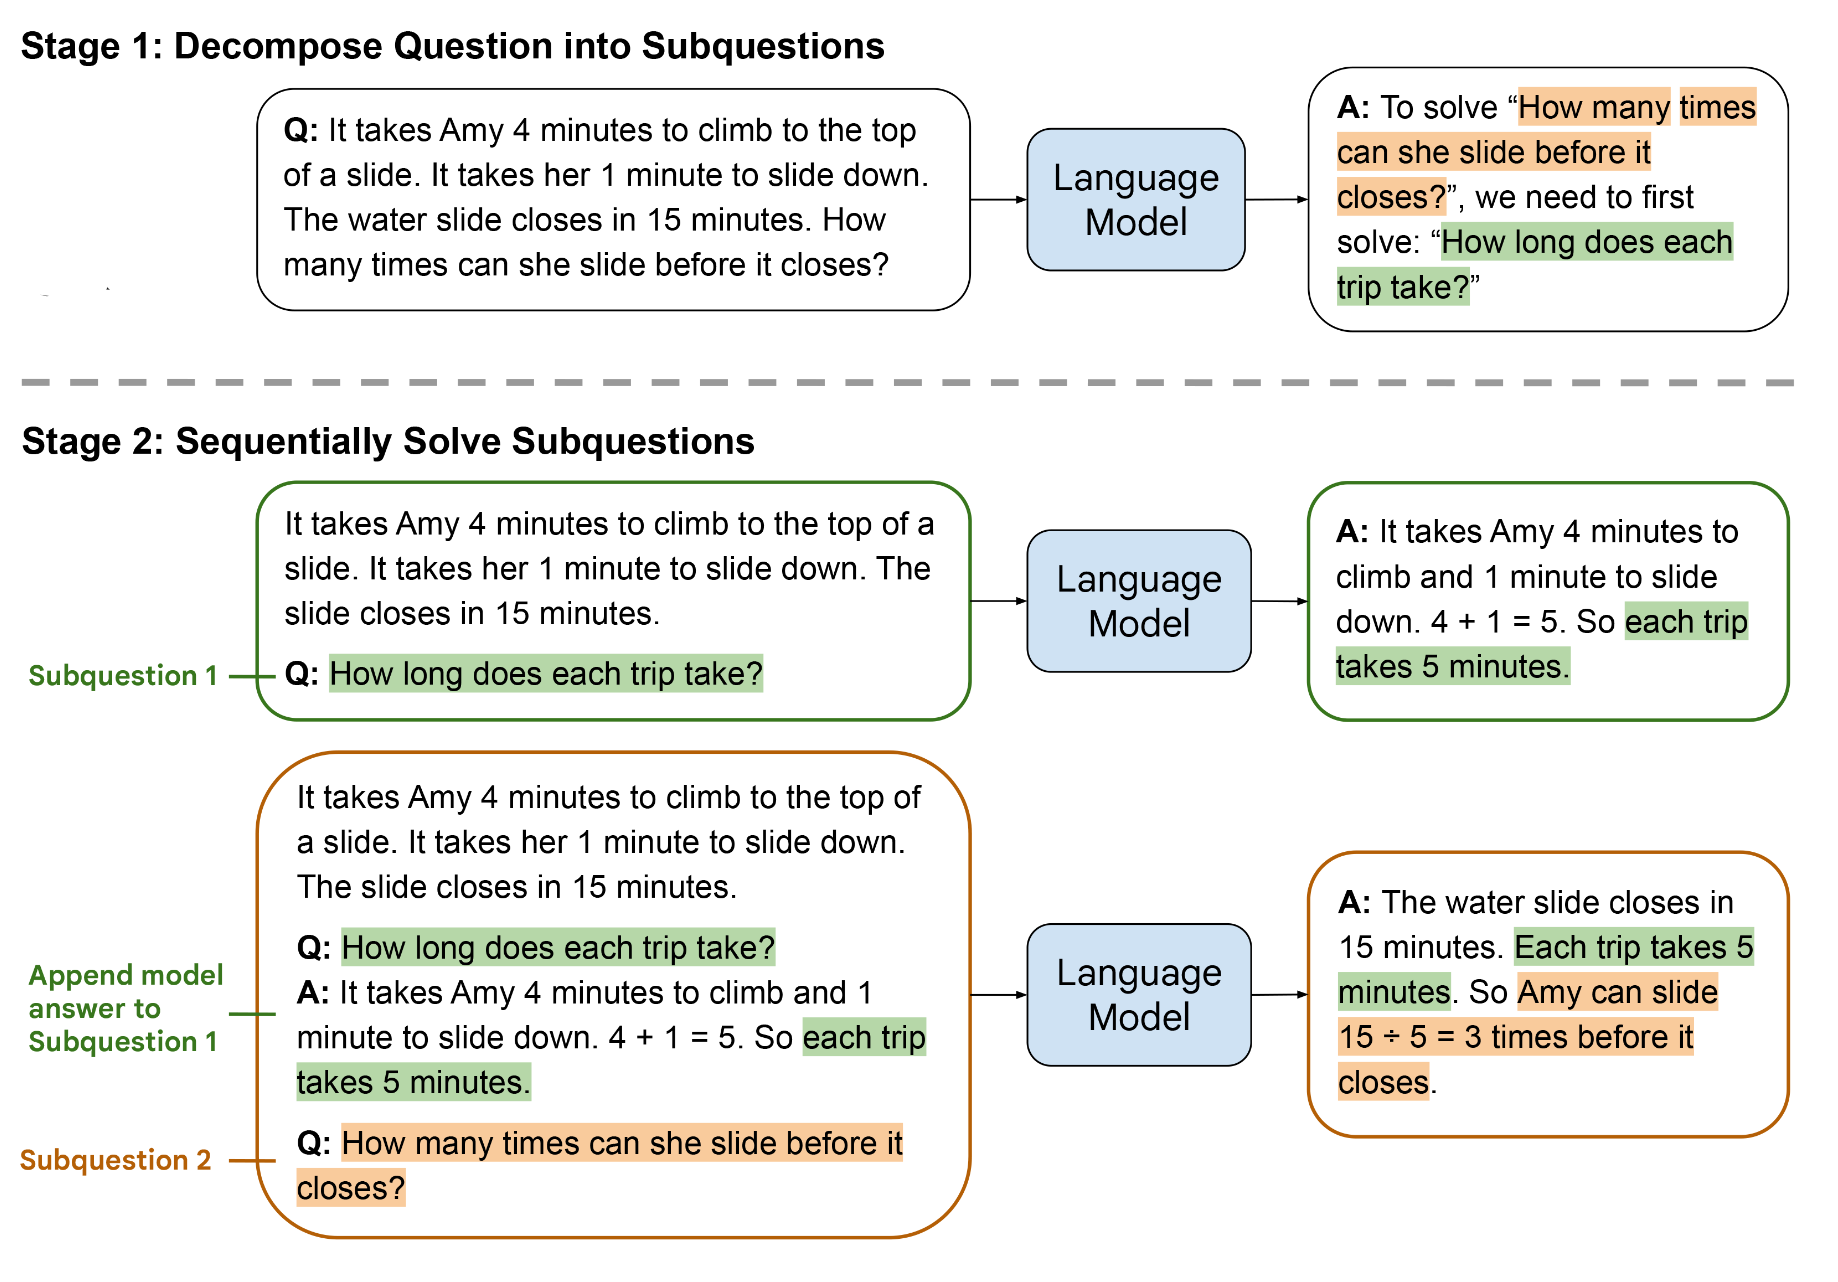
\includegraphics[height=6cm]{./p8.png}
\caption{\label{fig:orgef22c12}\tiny Least-to-most prompting solving a math word problem in two stages: (1) query the language model to decompose the problem into subproblems; (2) query the language model to sequentially solve the subproblems. The answer to the second subproblem is built on the answer to the first subproblem. The demonstration examples for each stage’s prompt are omitted in this illustration.}
\end{figure}
\end{frame}

\begin{frame}[label={sec:orgced2402}]{Lets Think Step by Step (Zero-Shot-CoT) \footfullcite{kojimaLargeLanguageModels2023}}
\begin{figure}[htbp]
\centering
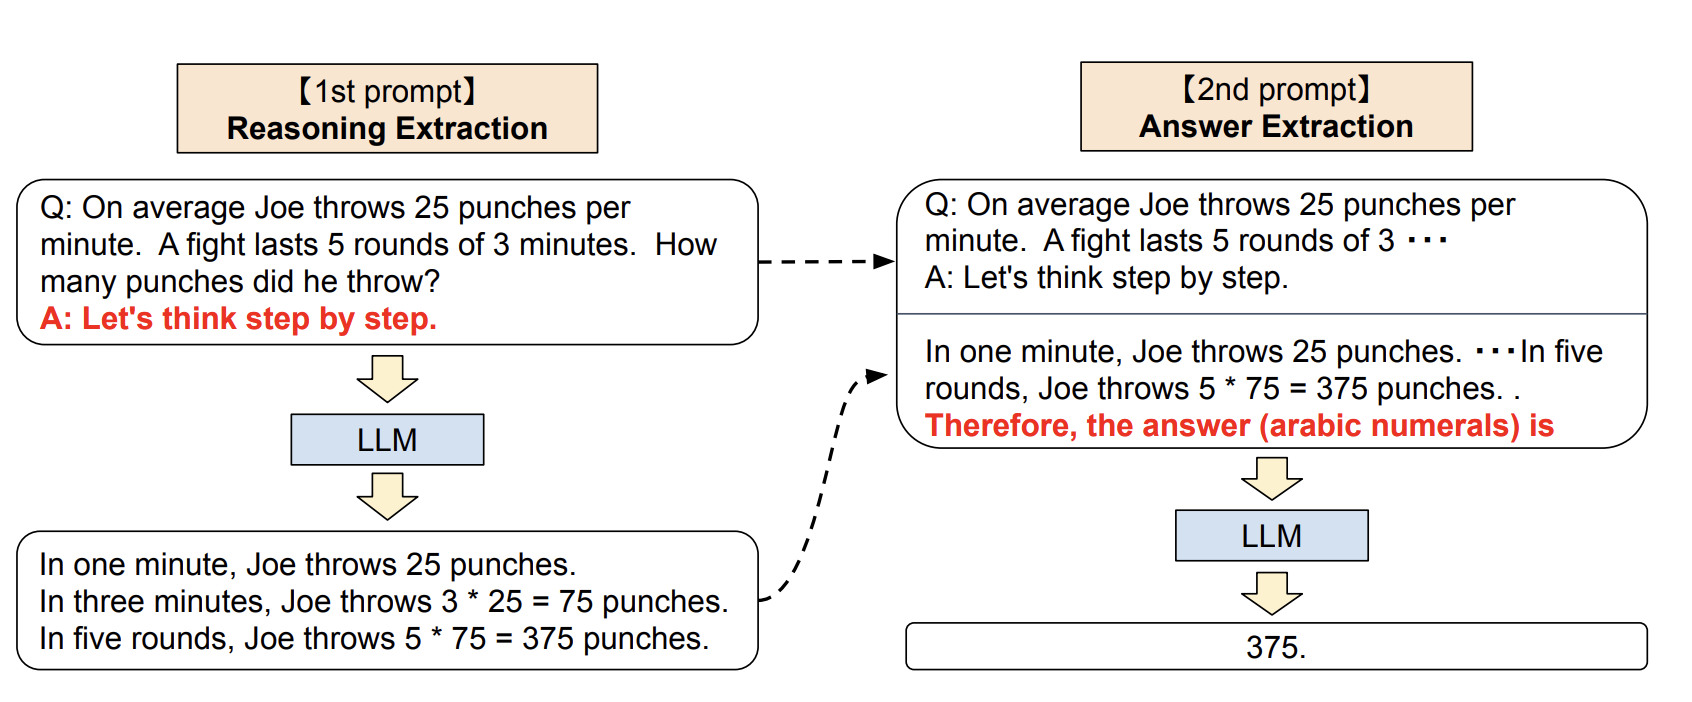
\includegraphics[width=.9\linewidth]{./p4.png}
\caption{\label{fig:org12ffdb9}Lets think step by step.}
\end{figure}
\end{frame}

\begin{frame}[label={sec:orgd94c884}]{Results}
\begin{figure}[htbp]
\centering
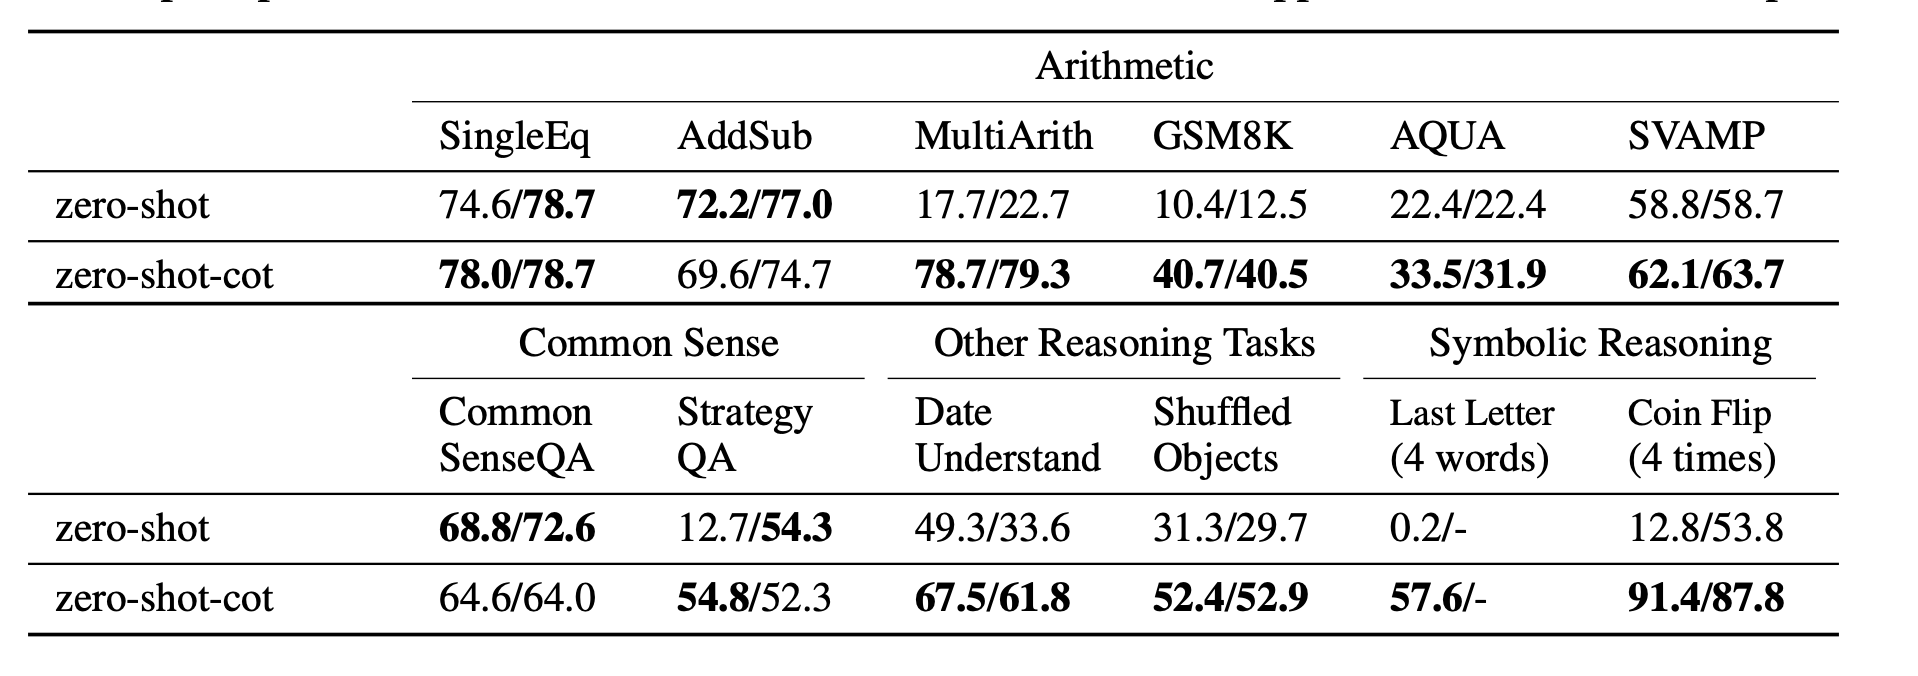
\includegraphics[width=.9\linewidth]{./p10.png}
\caption{\label{fig:org4ff6b03}Accuracy comparison of Zero-shot-CoT with Zero-shot on each tasks. The values on the left side of each task are the results of using answer extraction prompts depending on answer format.  The values on the right side are the result of additional experiment where standard answer prompt "The answer is" is used for answer extraction}
\end{figure}
\end{frame}

\begin{frame}[label={sec:org61651aa}]{Inference -- Scoring Function}
Channel Model \footfullcite{minNoisyChannelLanguage2022}

\begin{figure}[htbp]
\centering
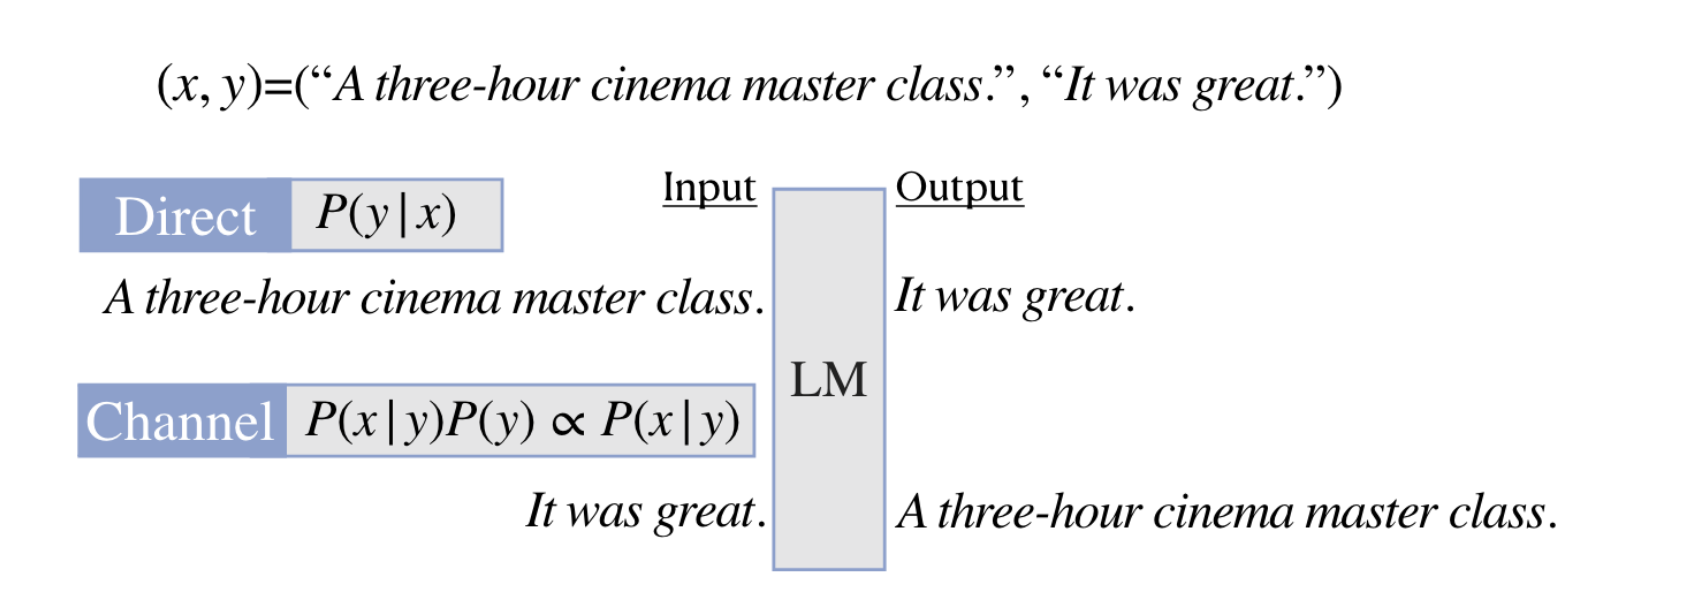
\includegraphics[width=.9\linewidth]{./p5.png}
\caption{\label{fig:org12bb484}Channel model.}
\end{figure}
\end{frame}

\section{Does ICL really learn something?}
\label{sec:orgbff0c2e}

\begin{frame}[label={sec:org21beb51},fragile]{No}
 \begin{itemize}
\item In \emph{Rethinking the Role of Demonstrations: What Makes In-Context Learning Work?} \footfullcite{minRethinkingRoleDemonstrations2022}, the authors show that ICL is not learning anything.
\item They use a random label \(y_{r} \in Y\) to replace the true label \(y_{i}\) for \(x_{i}\), and the model still works.
\item What really affects is the distribution of \(<x_{i}, y_{i}>\).
\end{itemize}

\begin{verbatim}
[ME]:
Review: Delicious food      Sentiment: Negative
Review: The food is awful   Sentiment: Positive
Review: Terrible dishes     Sentiment: Negative
Review: Good meal           Sentiment:

[AI]: Positive
\end{verbatim}
\end{frame}

\begin{frame}[label={sec:orgcf8e2b2}]{Yes}
\begin{itemize}
\item Ekin Akyurek \footfullcite{akyurekWhatLearningAlgorithm2023}
\begin{itemize}
\item Transformer-based in-context learners implement standard learning algorithms implicitly, by encoding smaller models in their activations, and updating these implicit models as new examples appear in the context.
\end{itemize}
\item Damai Dai \footfullcite{daiWhyCanGPT2022}
\begin{itemize}
\item Language models is meta-optimizers and understands ICL is a kind of implicit finetuning.
\end{itemize}
\end{itemize}
\end{frame}

\section{Conclusion}
\label{sec:org533377f}

\begin{frame}[label={sec:org66ba318}]{Conclusion}
\begin{itemize}
\item In-context learnig (ICL) difinition
\item Taxonomy of ICL
\item Relation between ICL and instruct
\item ICL in Training
\item ICL in Inference
\begin{itemize}
\item Demonstration Designing
\begin{itemize}
\item Selection and Order
\item Formatting
\end{itemize}
\item Scoring Function
\end{itemize}
\end{itemize}
\end{frame}

\section{Reference}
\label{sec:orgeb5d522}

\begin{frame}[allowframebreaks]{Reference}
\printbibliography
\end{frame}

\section{Examples}
\label{sec:org1525a82}

\begin{frame}[fragile,allowframebreaks]{Example}
 Over-fitting and over-smoothing are two main obstacles of developing deep Graph Convolutional Networks (GCNs) for node classification. In particular, over-fitting weakens the generalization ability on small dataset, while over-smoothing impedes model training by isolating output representations from the input features with the increase in network depth.  This paper proposes DropEdge, a novel and flexible technique to alleviate both issues. At its core, DropEdge randomly removes a certain number of edges from the input graph at each training epoch, acting like a data augmenter and also a message passing reducer. Furthermore, we theoretically demonstrate that DropEdge either reduces the convergence speed of over-smoothing or relieves the information loss caused by it. More importantly, our DropEdge is a general skill that can be equipped with many other backbone models (e.g.  GCN, ResGCN, GraphSAGE, and JKNet) for enhanced performance.  Extensive experiments on several benchmarks verify that DropEdge consistently improves the performance on a variety of both shallow and deep GCNs.  The effect of DropEdge on preventing over-smoothing is empirically visualized and validated as well.  Codes are released on \url{https://github.com/DropEdge/DropEdge}


\begin{verbatim}
[ME]:
Alice is Bob’s roommate. Make her node green.
[
["Alice", "is roommate", "Bob"],
["Alice", "#00FF00"]
]

In this paper, we question if self-supervised learning provides new properties to Vision Transformer (ViT) [19] that stand out compared to convolutional networks (convnets).  Beyond the fact that adapting self-supervised methods to this architecture works particularly well, we make the following observations: first, self-supervised ViT features contain explicit information about the semantic segmentation of an image, which does not emerge as clearly with supervised ViTs, nor with convnets. Second, these features are also excellent k-NN classifiers, reaching 78.3% top-1 on ImageNet with a small ViT. Our study also underlines the importance of momentum encoder [33], multi-crop training [10], and the use of small patches with ViTs. We implement our findings into a simple self-supervised method, called DINO, which we interpret as a form of self-distillation with no labels.  We show the synergy between DINO and ViTs by achieving 80.1% top-1 on ImageNet in linear evaluation with ViT-Base.
[
["Paper", "focus", "self-supervised learning properties of ViT"],
["ViT", "compared to", "convnets"],
["Self-supervised ViT", "observation", "contains explicit information about semantic segmentation"],
["Self-supervised ViT", "observation", "excellent k-NN classifiers"],
["Self-supervised ViT", "performance", "78.3% top-1 on ImageNet with a small ViT"],
["Momentum encoder", "importance", "self-supervised learning"],
["Multi-crop training", "importance", "self-supervised learning"],
["Small patches", "importance", "self-supervised learning with ViTs"],
["DINO", "implemented", "self-supervised method"],
["DINO", "interpretation", "self-distillation with no labels"],
["DINO", "synergy", "ViTs"],
["DINO and ViT-Base", "performance", "80.1% top-1 on ImageNet in linear evaluation"]
]

Over-fitting and over-smoothing are two main obstacles of developing deep Graph Convolutional Networks (GCNs) for node classification. In particular, over-fitting weakens the generalization ability on small dataset, while over-smoothing impedes model training by isolating output representations from the input features with the increase in network depth.  This paper proposes DropEdge, a novel and flexible technique to alleviate both issues. At its core, DropEdge randomly removes a certain number of edges from the input graph at each training epoch, acting like a data augmenter and also a message passing reducer. Furthermore, we theoretically demonstrate that DropEdge either reduces the convergence speed of over-smoothing or relieves the information loss caused by it. More importantly, our DropEdge is a general skill that can be equipped with many other backbone models (e.g.  GCN, ResGCN, GraphSAGE, and JKNet) for enhanced performance.  Extensive experiments on several benchmarks verify that DropEdge consistently improves the performance on a variety of both shallow and deep GCNs.  The effect of DropEdge on preventing over-smoothing is empirically visualized and validated as well.  Codes are released on https://github.com/DropEdge/DropEdge
[
["Over-fitting", "obstacle", "GCNs"],
["Over-smoothing", "obstacle", "GCNs"],
["GCNs", "purpose", "node classification"],
["DropEdge", "proposed for", "alleviating over-fitting and over-smoothing"],
["DropEdge", "function", "randomly removes edges"],
["DropEdge", "acts as", "data augmenter"],
["DropEdge", "acts as", "message passing reducer"],
["DropEdge", "effect", "reduces convergence speed of over-smoothing or relieves information loss"],
["DropEdge", "applicable to", "GCN"],
["DropEdge", "applicable to", "ResGCN"],
["DropEdge", "applicable to", "GraphSAGE"],
["DropEdge", "applicable to", "JKNet"],
["Experiments", "validate", "DropEdge"],
["DropEdge", "prevents", "over-smoothing"],
["Codes", "available at", "https://github.com/DropEdge/DropEdge"]
]

Pretrained large language models (LLMs) are widely used in many sub-fields of natural language processing (NLP) and generally known as excellent few-shot learners with task-specific exemplars. Notably, chain of thought (CoT) prompting, a recent technique for eliciting complex multi-step reasoning through step-bystep answer examples, achieved the state-of-the-art performances in arithmetics and symbolic reasoning, difficult system-2 tasks that do not follow the standard scaling laws for LLMs. While these successes are often attributed to LLMs’ ability for few-shot learning, we show that LLMs are decent zero-shot reasoners by simply adding “Let’s think step by step” before each answer. Experimental results demonstrate that our Zero-shot-CoT, using the same single prompt template, significantly outperforms zero-shot LLM performances on diverse benchmark reasoning tasks including arithmetics (MultiArith, GSM8K, AQUA-RAT, SVAMP), symbolic reasoning (Last Letter, Coin Flip), and other logical reasoning tasks (Date Understanding, Tracking Shuffled Objects), without any hand-crafted few-shot examples, e.g. increasing the accuracy on MultiArith from 17.7% to 78.7% and GSM8K from 10.4% to 40.7% with large-scale InstructGPT model (text-davinci002), as well as similar magnitudes of improvements with another off-the-shelf large model, 540B parameter PaLM. The versatility of this single prompt across very diverse reasoning tasks hints at untapped and understudied fundamental zero-shot capabilities of LLMs, suggesting high-level, multi-task broad cognitive capabilities may be extracted by simple prompting. We hope our work not only serves as the minimal strongest zero-shot baseline for the challenging reasoning benchmarks, but also highlights the importance of carefully exploring and analyzing the enormous zero-shot knowledge hidden inside LLMs before crafting finetuning datasets or few-shot exemplars.

[AI]: [
["Pretrained large language models", "widely used in", "many sub-fields of NLP"],
["LLMs", "known for", "excellent few-shot learning"],
["Chain of thought (CoT)", "a recent technique for", "eliciting complex multi-step reasoning"],
["CoT prompting", "achieved", "state-of-the-art performances in arithmetics and symbolic reasoning"],
["CoT prompting", "successes attributed to", "LLMs ability for few-shot learning"],
["Zero-shot-CoT", "outperforms", "zero-shot LLM performances on diverse benchmark reasoning tasks"],
["Zero-shot-CoT", "uses", "same single prompt template"],
["Zero-shot-CoT", "increases accuracy on MultiArith from 17.7% to 78.7% and GSM8K from 10.4% to 40.7% with large-scale InstructGPT model (text-davinci002)"],
["Zero-shot-CoT", "similar magnitudes of improvements", "with another off-the-shelf large model, 540B parameter PaLM"],
["Single prompt", "versatile across", "diverse reasoning tasks"],
["Zero-shot capabilities", "hidden inside LLMs", "untapped and understudied fundamental"],
["Zero-shot capabilities", "suggests high-level, multi-task broad cognitive capabilities", "may be extracted by simple prompting"],
["Importance", "carefully exploring and analyzing the enormous zero-shot knowledge", "hidden inside LLMs"],
["Hope", "work serves as", "minimal strongest zero-shot baseline for the challenging reasoning benchmarks"],
["Hope", "work highlights", "importance of exploring and analyzing the enormous zero-shot knowledge hidden inside LLMs"]
]

[ME]:
\end{verbatim}
\end{frame}
\end{document}